\documentclass{beamer}
%\usepackage{xspace}
\usepackage{amsmath,amssymb}
\usepackage{graphicx}
\usepackage{pgfpages}
%\pgfpagesuselayout{4 on 1}[a4paper,border shrink=5mm,landscape]
%\usepackage{psfrag}
%\usepackage[usenames,dvipsnames]{xcolor}
\usepackage{braket}
\usepackage{tikz}
\usetikzlibrary{graphs}
\usetikzlibrary{datavisualization}
\usetikzlibrary{datavisualization.formats.functions}
\usepackage{pgfplotstable}
\usepgfplotslibrary{patchplots}

\setbeamercovered{transparent}

\usetheme{Pittsburgh}
%\usetheme{default}

\setbeamertemplate{sidebar right}{}
\setbeamertemplate{footline}[frame number]
%\usefonttheme{professionalfonts}

%\usepackage{sansmathaccent}
%\usepackage{bm}

\newcommand{\backupbegin}{
   \newcounter{framenumberappendix}
   \setcounter{framenumberappendix}{\value{framenumber}}
}
\newcommand{\backupend}{
   \addtocounter{framenumberappendix}{-\value{framenumber}}
   \addtocounter{framenumber}{\value{framenumberappendix}} 
}

%\usepackage{unicode-math}
%%\setmainfont[SlantedFont={Latin Modern Roman Slanted},SlantedFeatures={Color=000000},
%%  SmallCapsFont={TeX Gyre Termes},SmallCapsFeatures={Letters=SmallCaps}]{XITS}
%\setmathfont[math-style=ISO,sans-style=upright]{XITS Math}
%\setmathfont[range={\mathcal,\mathbfcal}]{Latin Modern Math}

\usepackage{sfmath}

%\mathversion{sans}

\newcommand{\Tr}{\mathsf{Tr}}

\definecolor{redorange}{rgb}{1.0, .25, .25}
\definecolor{citation}{rgb}{.1, 0.8, .35}
\newcommand\emm[1]{\textcolor{redorange}{{#1}}}
\newcommand\numc[1]{\textcolor{citation}{{\bf #1}}}

%\newcommand\bm[1]{{\mbox{\boldmath $#1$}}}
\newcommand\bm[1]{{\mathbf{#1}}}
%\newcommand\bm[1]{{\bf #1}}
%\newcommand\bm[1]{\ensuremath{\boldsymbol{#1}}}
%\newcommand\bm[1]{{\textbf{\it #1}}}

%\title{Optimality of the three-input majority function on XOR games with nonlocal boxes}
%\title{How to characterize quantum physics by computer science}
\title{Operational characterization of quantum nonlocality}
\author{Ryuhei Mori}
%\institute{$\vcenter{\hbox{\includegraphics[width=30pt]{ELC_logo}}}$ Postdoctoral Fellow of ELC\\ $\vcenter{\hbox{\includegraphics[width=20pt]{titech_logo}}}$ Tokyo Institute of Technology}
\institute{Tokyo Institute of Technology}
\date{}



\begin{document}
\begin{frame}[plain]
\maketitle
\end{frame}

\begin{frame}{Motivation}
\begin{itemize}
\setlength{\itemsep}{3.0em}
\item Quantum physics has a beautiful mathematical representation.
\item But, we do not have any ``explanation'' for the quantum physics.
\item We need to find \emm{postulates} of quantum physics.\\
\vspace{1em}
Postulate: Similar to axiom in math. But, it must be testable by experiments, e.g.,
\begin{itemize}
\item Information cannot be transmitted faster than light.
\item A communication complexity is not always equal to 1.
\end{itemize}
\end{itemize}
\end{frame}

\if0
\begin{frame}{Quantum physics}
\begin{itemize}
\setlength{\itemsep}{3.5em}
\item There is no concept of ``quantum probability''.
%\item A probability is always what we know (which is represented by a tuple of non-negative real numbers whose sum is 1).
\item A probability is always expressed by a tuple of non-negative values with sum 1.
\item There are concepts of ``\emm{state}'' and ``\emm{measurement}''.
\begin{itemize}
\item State: Environment.
\item Measurement: Operation to a state for getting an outcome.
\item Probability of an output $a\in\mathcal{A}$ when a measurement $x\in\mathcal{X}$ is chosen is $P(a\mid x)$.
\end{itemize}
\end{itemize}
\end{frame}
\fi

\if0
\begin{frame}{State and measurement}
\begin{itemize}
\setlength{\itemsep}{3.0em}
\item In quantum physics, a state is represented by a PSD Hermitian matrix with trace 1.
\item In quantum physics, a measurement is represented by a tuple of PSD Hermitian matrices whose sum is the identity matrix.
\item When we apply a measurement $(P_1,\dotsc,P_m)$ to a state $\omega$, an outcome $i\in\{1,\dotsc,m\}$ is obtained with probability $\Tr(P_i\omega)$.
It is easy to confirm $\Tr(P_i\omega)\ge 0$ and $\sum_i \Tr(P_i\omega)=1$.
\item In the following, \emm{we do not consider the above concrete mathematical representation of states and measurements}.
\end{itemize}
\end{frame}
\fi


\begin{frame}{CHSH game~~\large[Bell 1964 \numc{11353}]\newline [Clauser, Horne, Shimony, Holt 1969 \numc{5779}]}
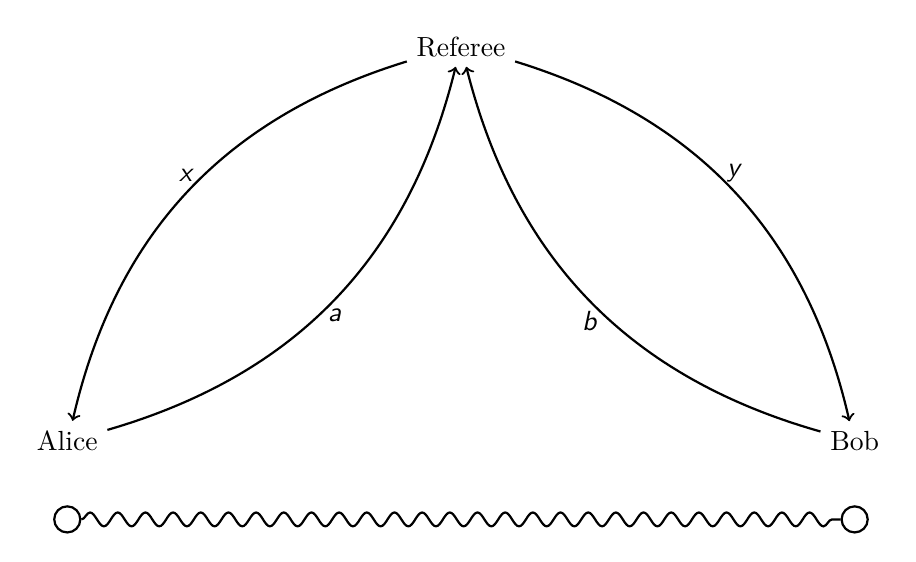
\begin{tikzpicture}
\node at (5,5) (R) {Referee};
\node at (0,0) (A) {Alice};
\node at (10,0) (B) {Bob};
\node at (0,-1)[circle,thick,draw] (As) {};
\node at (10,-1)[circle,thick,draw] (Bs) {};
\draw[->,thick] (R) edge[bend right] node[anchor=south, midway]{$x$} (A);
\draw[->,thick] (R) edge[bend left] node[anchor=south, midway]{$y$} (B);
\draw[->,thick] (A) edge[bend right] node[anchor=north, midway]{$a$} (R);
\draw[->,thick] (B) edge[bend left] node[anchor=north, midway]{$b$} (R);
\draw[thick,decorate,decoration=snake] (As) -- (Bs);
\end{tikzpicture}
%\includegraphics[width=30pt]{Alice_in_Wonderland.png}
\begin{center}
Alice and Bob win iff $\emm{a\oplus b = x\wedge y}$.
\end{center}
\end{frame}


\begin{frame}{CHSH winning probability}
\begin{itemize}
\setlength{\itemsep}{3.5em}
\item The maximum CHSH winning probability in \emm{classical physics} is $3/4=0.75$.\\
\begin{align*}
a_0\oplus b_0 &=0\\
a_0\oplus b_1 &=0\\
a_1\oplus b_0 &=0\\
a_1\oplus b_1 &=1
\end{align*}
%\begin{center}
%\begin{tikzpicture}
%\node at (0,0) {a0};
%\node at (2,2) {a1};
%\node at (2,0) {b0};
%\node at (0,2) {b1};
%\node[rotate=90] at (0,1) {$=$};
%\node at (1,0) {$=$};
%\node[rotate=90] at (2,1) {$=$};
%\node at (1,2) {$\ne$};
%\end{tikzpicture}
%\end{center}
\item The maximum CHSH winning probability in \emm{quantum physics} is $(2+\sqrt{2})/4\approx 0.854$
[Tsirelson 1980 \numc{1195}].
\end{itemize}
\end{frame}

\begin{frame}{Locality (Hidden variable model)}
\begin{center}
Joint preparation and independent measurements.
\end{center}
Probability distribution $P(a,b\mid x,y)$ is said to be \emm{local} if
\begin{equation*}
P(a, b\mid x,y) = \sum_{\lambda} P(\lambda) P(a\mid x, \lambda) P(b\mid y,\lambda).
\end{equation*}
\vspace{2em}
\begin{center}
Quantum physics allow \emm{nonlocal} behaviors.
\end{center}
\end{frame}

\if0
\begin{frame}{Einstein--Podolsky--Rosen (EPR) paradox}
\begin{equation*}
P(a, b\mid x,y) = \sum_{\lambda} P(\lambda) P(a\mid x, \lambda) P(b\mid y,\lambda).
\end{equation*}
$\iff$
there exists a joint distribution of $(\{a_x\}_{x\in X}, \{b_y\}_{y\in Y})$.

\begin{center}
\Large
$\Downarrow$

\vspace{1.0em}
\normalsize
In quantum physics,
$a_0,a_1,b_0,b_1$ \emm{cannot \textit{exists}} simultaneously.

\vspace{1.0em}
\Large
$\Downarrow$

\vspace{1.0em}
\normalsize
In quantum physics,
position and momentum \emm{cannot \textit{exists}} simultaneously.
\end{center}

[Einstein, Podolsky, Rosen 1935, \numc{15771}]
\end{frame}
\fi

\if0
\begin{frame}{Quantum CHSH probability}
\begin{equation*}
\ket{\psi} = \frac1{\sqrt{2}}\left(\ket{0}\ket{0} + \ket{1}\ket{1}\right)
\end{equation*}
\begin{equation*}
\ket{\phi_\theta} = \cos(\theta) \ket{0} + \sin(\theta) \ket{1}
\end{equation*}
\begin{align*}
\bigl|\bra{\phi_{\theta_A}}\bra{\phi_{\theta_B}}\ket{\psi}\bigr|^2
&=\Bigl|\frac1{\sqrt{2}}\left(\cos(\theta_A)\cos(\theta_B) + \sin(\theta_A)\sin(\theta_B)\right)\Bigr|^2\\
&=\frac12\cos^2(\theta_A-\theta_B)
\end{align*}
\end{frame}

\begin{frame}{Quantum CHSH probability}
\begin{center}
\begin{tikzpicture}
\draw[->,thick] (0,0) to (2,0);
\draw[->,thick] (0,0) to (0,2);
\draw[->,dashed,thick] (0,0) to ({2*cos(45)},{2*sin(45)});
\draw[->,dashed,thick] (0,0) to ({2*cos(135)},{2*sin(135)});;
\draw[->,thick] (5,0) to ({5+2*cos(22.5)},{2*sin(22.5)});
\draw[->,thick] (5,0) to ({5+2*cos(112.5)},{2*sin(112.5)});
\draw[->,dashed,thick] (5,0) to ({5+2*cos(-22.5)},{2*sin(-22.5)});
\draw[->,dashed,thick] (5,0) to ({5+2*cos(67.5)},{2*sin(67.5)});;
\end{tikzpicture}
\end{center}
\begin{align*}
\theta_A^{x=0} &= 0, & \theta_A^{x=1} &= \pi/4, &
\theta_B^{y=0} &= \pi/8, & \theta_B^{y=1} &= -\pi/8
\end{align*}
For any $x\in\{0,1\}, y\in\{0,1\}$, the winning probability is
\begin{equation*}
\cos^2\left(\frac{\pi}8\right)
=
\frac{2+\sqrt{2}}4
\approx 0.854
\end{equation*}
\end{frame}
\fi

\begin{frame}{Two-party statistics}
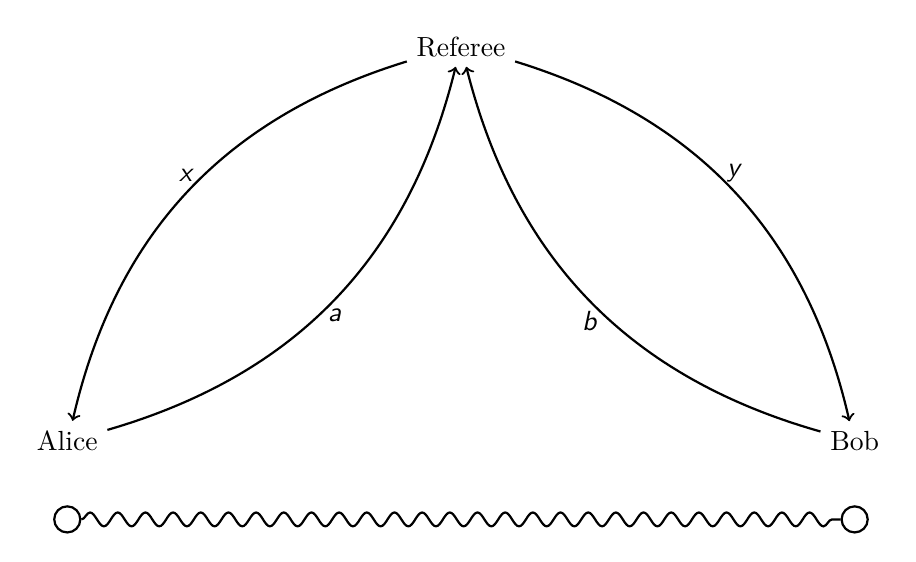
\begin{tikzpicture}
\node at (5,5) (R) {Referee};
\node at (0,0) (A) {Alice};
\node at (10,0) (B) {Bob};
\node at (0,-1)[circle,thick,draw] (As) {};
\node at (10,-1)[circle,thick,draw] (Bs) {};
\draw[->,thick] (R) edge[bend right] node[anchor=south, midway]{$x$} (A);
\draw[->,thick] (R) edge[bend left] node[anchor=south, midway]{$y$} (B);
\draw[->,thick] (A) edge[bend right] node[anchor=north, midway]{$a$} (R);
\draw[->,thick] (B) edge[bend left] node[anchor=north, midway]{$b$} (R);
\draw[thick,decorate,decoration=snake] (As) -- (Bs);
\end{tikzpicture}
%\includegraphics[width=30pt]{Alice_in_Wonderland.png}
\begin{equation*}
P(a,b\mid x,y), \hspace{2em} \forall a,b\in\{0,1\}, x,y\in\{0,1\}
\end{equation*}
\end{frame}

\begin{frame}{No-signaling condition}
The marginal distribution of $a$ ($b$) \emm{cannot depend on} $y$ ($x$), respectively.
\begin{align*}
\sum_{b\in\{0,1\}} P(a,b\mid x,0) &= \sum_{b\in\{0,1\}} P(a,b\mid x,1),\qquad\forall a,\,x\in\{0,1\}\\
\sum_{a\in\{0,1\}} P(a,b\mid 0,y) &= \sum_{a\in\{0,1\}} P(a,b\mid 1,y),\qquad\forall b,\,y\in\{0,1\}.
\end{align*}
\end{frame}

\begin{frame}{The 8-dimensional linear space and no-signaling polytope}
\small
\begin{align*}
\sum_{a\in\{0,1\},\,b\in\{0,1\}} P(a,b\mid x,y) = 1,\qquad x\in\{0,1\},\, y\in\{0,1\}.
\end{align*}
\begin{align*}
\sum_{b\in\{0,1\}} P(0,b\mid 0,0) &= \sum_{b\in\{0,1\}} P(0,b\mid 0,1)\\
\sum_{b\in\{0,1\}} P(0,b\mid 1,0) &= \sum_{b\in\{0,1\}} P(0,b\mid 1,1)\\
\sum_{a\in\{0,1\}} P(a,0\mid 0,0) &= \sum_{a\in\{0,1\}} P(a,0\mid 1,0)\\
\sum_{a\in\{0,1\}} P(a,0\mid 0,1) &= \sum_{a\in\{0,1\}} P(a,0\mid 1,1).
\end{align*}

\vspace{.5em}
\begin{center}
$16-8=\emm{8}$-dimensional linear space.
\end{center}
\end{frame}

\begin{frame}{No-signaling polytope}
\centering
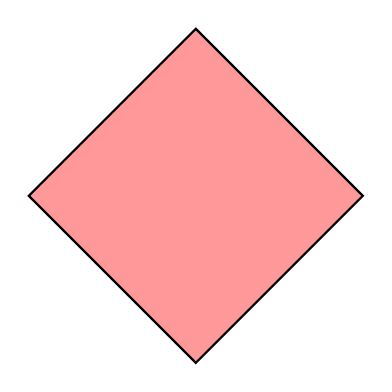
\begin{tikzpicture}
\draw [rotate=45, thick, red!40, fill, draw=black] (-1.5,-1.5) rectangle  (1.5,1.5);
%\draw [thick, green!40, fill] (-1.061,-1.061) rectangle  (1.061,1.061);
\end{tikzpicture}
\end{frame}

\begin{frame}{Local polytope}
\emm{Deterministic} choice
\begin{align*}
a&=A(x),& b&=B(y).
\end{align*}

Local polytope
\begin{align*}
\mathsf{conv}\left(\left\{\left\{P(a,b\mid x,y)=\delta_{(a,b),(A(x),B(y))}\right\}_{a,b,x,y}\mid A, B\in\{0,1\}^{\{0,1\}}\right\}\right).
\end{align*}

\end{frame}

\begin{frame}{No-signaling polytope and local polytope}
\centering
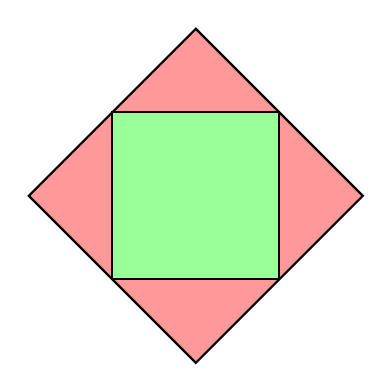
\begin{tikzpicture}
%\draw [fill, black!50] (0,0) circle [radius=1.5cm];
%\draw (-1.061,-1.061) rectangle (1.061,1.061);
\draw [rotate=45, thick, red!40, fill, draw=black] (-1.5,-1.5) rectangle  (1.5,1.5);
\draw [thick, green!40, fill, draw=black] (-1.061,-1.061) rectangle  (1.061,1.061);
%\draw [dashed,thick] (-1.061*2, 1.5) to (1.061*2, 1.5) node[right] {CHSH probability $ \approx 0.854$};
%\draw [dashed,thick] (-1.061*2, 1.061*2) to (1.061*2, 1.061*2) node[right] {CHSH probability $ = 1$};
%\draw (5.5,-0.5) node [align=left, text width = 5.9cm ] (T) {$BNL;RNO3X$K$h$C$F@8@.$5$l$kAj4X$N=89g!#(B\\ \textbf{$B$3$N=89g$r!VA`:nE*0UL#$N$"$k>r7o$G!WFCD'IU$1$?$$(B}};
%\draw [->,thick] (2.5,-0.2) node [right, align=left, text width = 5.9cm ] {$BNL;RNO3X$K$h$C$F@8@.$5$l$kAj4X$N=89g!#(B\\ \textbf{$B$3$N=89g$r!VA`:nE*0UL#$N$"$k>r7o$G!WFCD'IU$1$?$$(B}} to (1.5,0.2);
%\draw [-{Stealth[length=2.5mm]},thick] (T.west) to (1.5,-0.2);
%\draw [-{Stealth[length=2.5mm]},thick] (-2.5,0.5) node [left, align=left, text width = 5.2cm ] {No-signaling $B>r7o$N$_$rK~$?$9Aj4X$N=89g(B} to (-1.85,0.3);
\end{tikzpicture}
\end{frame}

\begin{frame}{CHSH inequality: Facets of the local polytope}
\begin{align*}
\emm{\sum_{a\oplus b=x\wedge y} P(a,b\mid x,y) }\ &\emm{\le 3},&
\sum_{a\oplus b\ne x\wedge y} P(a,b\mid x,y) &\le 3\\
\sum_{a\oplus b=\overline{x}\wedge y} P(a,b\mid x,y) &\le 3,&
\sum_{a\oplus b\ne \overline{x}\wedge y} P(a,b\mid x,y) &\le 3\\
\sum_{a\oplus b=x\wedge \overline{y}} P(a,b\mid x,y) &\le 3,&
\sum_{a\oplus b\ne x\wedge \overline{y}} P(a,b\mid x,y) &\le 3\\
\sum_{a\oplus b=\overline{x}\wedge \overline{y}} P(a,b\mid x,y) &\le 3,&
\sum_{a\oplus b\ne \overline{x}\wedge \overline{y}} P(a,b\mid x,y) &\le 3
\end{align*}
 CHSH inequality [{Clauser, Horne, Shimony, Holt} 1969 \numc{5779}].

CHSH inequality is the only non-trivial facets [Froissard 1981 \numc{81}], [Fine 1982 \numc{845}].
\end{frame}



\begin{frame}{No-signaling condition admits CHSH probability 1}
%\begin{align*}
%P(a = 0, b = 0\mid x=0, y = 0) &=
%P(a = 1, b = 1\mid x=0, y = 0) = 1/2\\
%P(a = 0, b = 0\mid x=0, y = 1) &=
%P(a = 1, b = 1\mid x=0, y = 1) = 1/2\\
%P(a = 0, b = 0\mid x=1, y = 0) &=
%P(a = 1, b = 1\mid x=1, y = 0) = 1/2\\
%P(a = 0, b = 1\mid x=1, y = 1) &=
%P(a = 1, b = 0\mid x=1, y = 1) = 1/2
%\end{align*}

\begin{align*}
P(0, 0\mid 0, 0) &=
P(1, 1\mid 0, 0) = 1/2\\
P(0, 0\mid 0, 1) &=
P(1, 1\mid 0, 1) = 1/2\\
P(0, 0\mid 1, 0) &=
P(1, 1\mid 1, 0) = 1/2\\
P(0, 1\mid 1, 1) &=
P(1, 0\mid 1, 1) = 1/2
\end{align*}

\vspace{1em}
\begin{center}
[Popescu and  Rohrlich 1994 \numc{955}]
\end{center}
\end{frame}

\begin{frame}{No-signaling polytope, local polytope and quantum correlation}
\centering
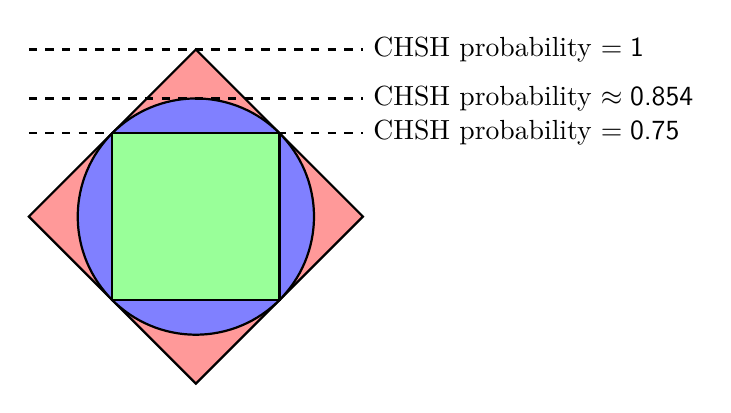
\begin{tikzpicture}
%\draw (-1.061,-1.061) rectangle (1.061,1.061);
\draw [rotate=45, thick, red!40, fill, draw=black] (-1.5,-1.5) rectangle  (1.5,1.5);
\draw [blue!50, fill, thick, draw=black] (0,0) circle [radius=1.5cm];
\draw [thick, green!40, fill, draw=black] (-1.061,-1.061) rectangle  (1.061,1.061);
\draw [dashed,thick] (-1.061*2, 1.5) to (1.061*2, 1.5) node[right] {CHSH probability $ \approx 0.854$};
\draw [dashed,thick] (-1.061*2, 1.061*2) to (1.061*2, 1.061*2) node[right] {CHSH probability $ = 1$};
\draw [dashed,thick] (-1.061*2, 1.061) to (1.061*2, 1.061) node[right] {CHSH probability $ = 0.75$};
%\draw (5.5,-0.5) node [align=left, text width = 5.9cm ] (T) {$BNL;RNO3X$K$h$C$F@8@.$5$l$kAj4X$N=89g!#(B\\ \textbf{$B$3$N=89g$r!VA`:nE*0UL#$N$"$k>r7o$G!WFCD'IU$1$?$$(B}};
%\draw [->,thick] (2.5,-0.2) node [right, align=left, text width = 5.9cm ] {$BNL;RNO3X$K$h$C$F@8@.$5$l$kAj4X$N=89g!#(B\\ \textbf{$B$3$N=89g$r!VA`:nE*0UL#$N$"$k>r7o$G!WFCD'IU$1$?$$(B}} to (1.5,0.2);
%\draw [-{Stealth[length=2.5mm]},thick] (T.west) to (1.5,-0.2);
%\draw [-{Stealth[length=2.5mm]},thick] (-2.5,0.5) node [left, align=left, text width = 5.2cm ] {No-signaling $B>r7o$N$_$rK~$?$9Aj4X$N=89g(B} to (-1.85,0.3);
\end{tikzpicture}

\vspace{1em}
\centering
Question:

\vspace{.5em}
\bfseries
Why does quantum physics prohibits CHSH probability greater than $\mathbf{(2+\sqrt{2})/4\approx0.854}$ ?
\end{frame}

\if0
\begin{frame}{Summary}
No-signaling polytope
\begin{itemize}
\item 16 facets.
\item 24 vertices (16 local vertices + 8 PR boxes).
\item CHSH probability at most 1.
\end{itemize}

\vspace{2em}
Local polytope
\begin{itemize}
\item 16 vertices.
\item 24 facets (16 trivial facets + \emm{8 CHSH facets}).
\item CHSH probability at most 3/4.
\end{itemize}

\vspace{2em}
Quantum correlation
\begin{itemize}
\item CHSH probability at most $\emm{(2+\sqrt{2})/4}$.
\end{itemize}
\end{frame}

\begin{frame}{Reference}

\vspace{2em}
\begin{center}
\LARGE
{\Huge Bell nonlocality}

\vspace{.5em}
N.~Brunner, D.~Cavalcanti, S.~Pironio, V.~Scarani, and S.~Wehner,

\vspace{.5em}
Reviews of Modern Physics, 86, 419, 2014.\\
\numc{504}

\vspace{3em}
\normalsize
An extremely well-written survey paper.
\end{center}

\end{frame}

\section{The polytopes on general alphabets}

%\frame{\insertsection}

\begin{frame}{General alphabet}
\begin{equation*}
P(a,b\mid x,y), \hspace{2em} \forall a,b\in\{1,2,\dotsc,\Delta\}, x,y\in\{1,2,\dotsc,m\}
\end{equation*}

\vspace{1em}
The dimension is
\begin{align*}
&\Delta^2m^2-m^2-2(\Delta-1)m(m-1)\\
&=2(\Delta-1)m + (\Delta-1)^2m^2\\
&=((\Delta-1)m+1)^2-1
\end{align*}
\end{frame}

\begin{frame}{No-signaling polytope and local polytope in general case}
No-signaling polytope
\begin{itemize}
\item $\Delta^2m^2$ facets.
\item $8(2^{m-1}-1)^2$ vertices for $\Delta=2$, $m=*$.
\item $8(2^{\Delta-1}-1)^2$ vertices for $\Delta=*$, $m=2$.
\item \emm{?} vertices in general.
\end{itemize}

\vspace{2em}
Local polytope
\begin{itemize}
\item $\Delta^{2m}$ vertices.
\item 684 facets for $\Delta=2$, $m=3$ (36 trivial facets, 72 CHSH facets, 576 equivalent \emm{new facets}) [Froissard 1981 \numc{74}].
\item \emm{?} facets in general (even for $\Delta=2$, $m=4$).
\end{itemize}
\end{frame}

\begin{frame}{Correlations for $\Delta=2$}
\begin{align*}
m_{x=i} &:= P(a=0\mid x=i) - P(a=1\mid x=i)\\
m_{y=j} &:= P(b=0\mid y=j) - P(b=1\mid y=j)\\
m_{(x,y)=(i,j)} &:= P(a=b\mid x=i, y=j) - P(a\ne b\mid x=i, y=j)\\
\end{align*}
\begin{equation*}
\begin{matrix}
& m_{x=0} & m_{x=1}\\
m_{y=0} & m_{xy=00} & m_{xy=10}\\
m_{y=1} & m_{xy=01} & m_{xy=11}\\
\end{matrix}
\end{equation*}
\end{frame}

\begin{frame}{Local polytope for $\Delta=2$}
\begin{align*}
&\mathsf{conv}\left\{
\begin{bmatrix}
1&s(0)&s(1)\\
t(0)&t(0)s(0)&t(0)s(1)\\
t(1)&t(1)s(0)&t(1)s(1)
\end{bmatrix}
\mid
s,t\in\{+1,-1\}^m
\right\}\\
&=
\mathsf{conv}\left\{
\begin{bmatrix}
1\\
t(0)\\
t(1)
\end{bmatrix}
\begin{bmatrix}
1&
s(0)&
s(1)
\end{bmatrix}
\mid
s,t\in\{+1,-1\}^m
\right\}\\
\end{align*}
\end{frame}

\begin{frame}{Cut polytope}
\begin{align*}
\mathsf{CUT}(G) := \mathsf{conv}\left\{e^S\mid S\subseteq V(G)\right\}
\end{align*}
where
\begin{align*}
e^S_{uv} =
\begin{cases}
+1,& u\in S, v\in S \text{ or } u\notin S, v\notin S\\
-1,& u\in S, v\notin S \text{ or } u\notin S, v\in S\\
\end{cases}
\end{align*}

\vspace{1em}
\begin{equation*}
L_{\Delta=2,m}
=
\mathsf{CUT}(K_{1,m,m})
\end{equation*}

[Avis, Imai, Ito, and Sasaki 2004 \numc{11}]
\end{frame}

\begin{frame}{XOR game}
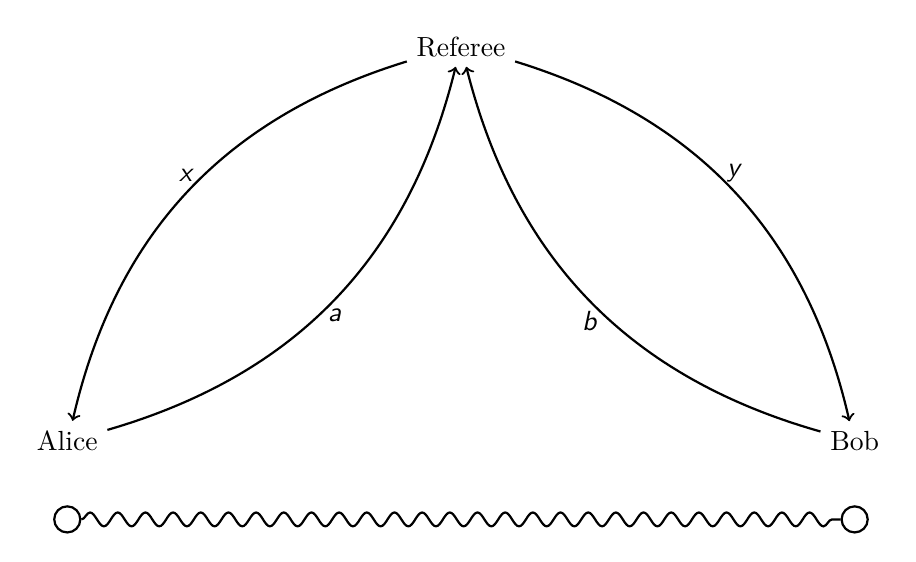
\begin{tikzpicture}
\node at (5,5) (R) {Referee};
\node at (0,0) (A) {Alice};
\node at (10,0) (B) {Bob};
\node at (0,-1)[circle,thick,draw] (As) {};
\node at (10,-1)[circle,thick,draw] (Bs) {};
\draw[->,thick] (R) edge[bend right] node[anchor=south, midway]{$x$} (A);
\draw[->,thick] (R) edge[bend left] node[anchor=south, midway]{$y$} (B);
\draw[->,thick] (A) edge[bend right] node[anchor=north, midway]{$a$} (R);
\draw[->,thick] (B) edge[bend left] node[anchor=north, midway]{$b$} (R);
\draw[thick,decorate,decoration=snake] (As) -- (Bs);
\end{tikzpicture}
%\includegraphics[width=30pt]{Alice_in_Wonderland.png}
\begin{center}
Alice and Bob win iff $\emm{a\oplus b = f(x,y)}$.
\end{center}
\end{frame}

\begin{frame}{Correlation space}
\begin{equation*}
\begin{matrix}
& m_{x=0} & m_{x=1}\\
m_{y=0} & m_{xy=00} & m_{xy=10}\\
m_{y=1} & m_{xy=01} & m_{xy=11}\\
\end{matrix}
\qquad
\Rightarrow
\qquad
\begin{matrix}
 m_{xy=00} & m_{xy=10}\\
 m_{xy=01} & m_{xy=11}\\
\end{matrix}
\end{equation*}

\vspace{1em}
\begin{align*}
CNS &= [-1,+1]^{m^2}\\
CL &= \mathsf{CUT}(K_{m,m})\\
CQ &= \Bigl\{ \{m_{xy} = \langle v_x, w_y\rangle\}_{x,y\in[m]}\mid\\
&\qquad v_x\in\mathbb{R}^{2m}, w_y\in\mathbb{R}^{2m}, \|v_x\|_2=\|w_y\|_2=1\Bigr\}.
\end{align*}
[Tsirelson 1980 \numc{1081}]
\end{frame}

\begin{frame}{Open problem}
\begin{itemize}
\setlength{\itemsep}{30pt}
\item Facets of local polytope, e.g., $\Delta=2$, \emm{$m=4$}.
\item Facets of local polytope in correlation space
(for $m=4$, 27968 facets, 15 types of inequalities [Hoban 2012]. Some relationship with [Gubeladze and Love 2014] ?)
%\item Vertices of no-signaling polytope
%\item Volumes of the polytopes
\end{itemize}
\end{frame}
\fi

\section{Trivial communication complexity with nonlocal boxes}

\if0
\begin{frame}{CHSH game and CHSH inequality}
%\begin{enumerate}
%\item Alice and Bob can share arbitrary state.
%\item Referee sends a bit $x$ to Alice and a bit $y$ to Bob.
%\item Alice and Bob send their answers $a$ and $b$ to the Referee (a measurement of the shared state is allowed).
%\item Alice and Bob win iff $a\oplus b = x \wedge y$.
%\end{enumerate}
\begin{center}
What is the maximum probability of winning ?
\begin{equation*}
\mathsf{CHSH}:= \sum_{(x,y)\in\{0,1\}^2} \Pr(m^A_x \oplus m^B_y = x\wedge y)
\end{equation*}
\begin{itemize}
\item Classical theory (hidden variable theory): $3$
 [{Clauser, Horne, Shimony, and Holt} 1969 \numc{4631}]
\item Quantum theory: $\emm{2+\sqrt{2}}\approx 3.414$ [Tsirelson 1980 \numc{927}]
\item PR box (gbit with $\otimes_{\max}$): $4$ [Popescu and  Rohrlich 1994 \numc{672}]
\end{itemize}
\end{center}
\end{frame}

\begin{frame}{PR box}
\begin{align*}
\Pr(m^{A}_0 = 0, m^{B}_0 = 0) &= 1/2,&
\Pr(m^{A}_0 = 1, m^{B}_0 = 1) &= 1/2\\
\Pr(m^{A}_0 = 0, m^{B}_1 = 0) &= 1/2,&
\Pr(m^{A}_0 = 1, m^{B}_1 = 1) &= 1/2\\
\Pr(m^{A}_1 = 0, m^{B}_0 = 0) &= 1/2,&
\Pr(m^{A}_1 = 1, m^{B}_0 = 1) &= 1/2\\
\Pr(m^{A}_1 = 0, m^{B}_1 = 1) &= 1/2,&
\Pr(m^{A}_1 = 1, m^{B}_1 = 0) &= 1/2
\end{align*}

\begin{center}
PR box satisfies the \emm{no-signaling} principle.
\end{center}
\end{frame}
\fi

\begin{frame}{Topics}
\begin{itemize}
\setlength{\itemsep}{1.5em}
\item $p_\mathsf{CHSH}=\emm{1} \qquad \Longrightarrow$ Communication complexity (CC) of arbitrary function is 1 bit.\\
 {\small [van Dam 2013 (quant-ph/0501159) (Ph.D. thesis 1999) \numc{168}]}
\item $p_\mathsf{CHSH}>\emm{(3+\sqrt{6})/6\approx 0.908} \qquad \Longrightarrow$ CC of arbitrary function is 1 bit.\\
{\small [Brassard, Buhrman, Linden, M\'ethot, Tapp, Unger 2006 \numc{250}]}
\item $p_\mathsf{CHSH}>\emm{(2+\sqrt{2})/4\approx 0.854} \qquad \Longrightarrow$ Information causality is violated.\\
{\small [Paw\l owki, Paterek, Kaszlikowski, Scarani, Winter, Zukowki 2009 \numc{375}]}
\item Brassard et al.'s result cannot be improved by generalizations of their techniques [Mori 2016].
\end{itemize}
\end{frame}

\begin{frame}{Nonlocal box}
\centering
Abstract device with two input ports and two output ports.
%\begin{equation*}
%P(a,b\mid x,y)
%\end{equation*}
\centering
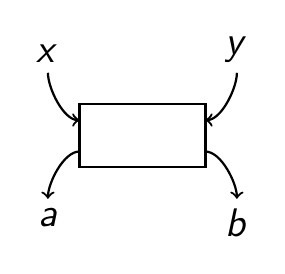
\begin{tikzpicture}[scale=0.4]
\draw[thick] (0,0) rectangle (4,2);
\draw[->,thick] (0, 0.5) .. controls +(left:5mm) and +(up:5mm) .. (-1,-1) node[at end, below] {\Large $a$};
\draw[->,thick] (4, 0.5) .. controls +(right:5mm) and +(up:5mm) .. (5,-1) node[at end, below] {\Large $b$};
\draw[<-,thick] (0, 1.5) .. controls +(left:5mm) and +(down:5mm) .. (-1,3) node[at end, above] {\Large $x$};
\draw[<-,thick] (4, 1.5) .. controls +(right:5mm) and +(down:5mm) .. (5,3) node[at end, above] {\Large $y$};
\end{tikzpicture}

\emm{Isotropic} nonlocal box
\begin{align*}
P(a,b\mid x,y) =
\begin{cases}
\frac{p_\mathsf{CHSH}}2,& \text{if } a\oplus b = x\wedge y\\
\frac{1-p_\mathsf{CHSH}}2,& \text{if } a\oplus b \ne x\wedge y.
\end{cases}
\end{align*}

\vspace{.5em}
This does not lose generality since
\begin{align*}
x\wedge y &= (x\oplus r_1)\wedge(y\oplus r_2) \oplus x\wedge r_2 \oplus r_1\wedge y \oplus r_1\wedge r_2\\
&= \emm{a \oplus b\oplus e} \oplus x\wedge r_2 \oplus r_1\wedge y \oplus r_1\wedge r_2\\
&= (\emm{a} \oplus x\wedge r_2 \oplus r_1\wedge r_2) \oplus (\emm{b}\oplus r_1\wedge y) \oplus \emm{e}\\
\end{align*}
\end{frame}

\begin{frame}{XOR game}
\centering
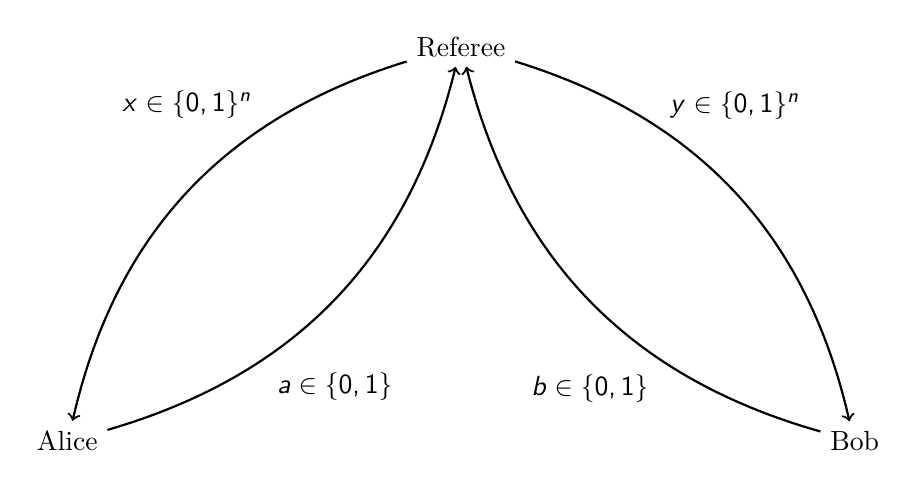
\begin{tikzpicture}
\node at (5,5) (R) {Referee};
\node at (0,0) (A) {Alice};
\node at (10,0) (B) {Bob};
%\node at (0,-1)[circle,thick,draw] (As) {};
%\node at (10,-1)[circle,thick,draw] (Bs) {};
\draw[->,thick] (R) edge[bend right] node[anchor=south, midway, above=.8cm]{$x\in\{0,1\}^n$} (A);
\draw[->,thick] (R) edge[bend left] node[anchor=south, midway, above=.8cm]{$y\in\{0,1\}^n$} (B);
\draw[->,thick] (A) edge[bend right] node[anchor=north, midway, below=.8cm]{$a\in\{0,1\}$} (R);
\draw[->,thick] (B) edge[bend left] node[anchor=north, midway, below=.8cm]{$b\in\{0,1\}$} (R);
%\draw[thick,decorate,decoration=snake] (As) -- (Bs);
\end{tikzpicture}

\vspace{.5em}
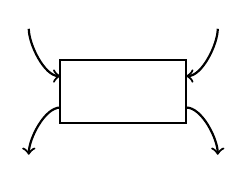
\begin{tikzpicture}[scale=0.4]
\draw[thick] (0,0) rectangle (4,2);
\draw[->,thick] (0, 0.5) .. controls +(left:5mm) and +(up:5mm) .. (-1,-1);
\draw[->,thick] (4, 0.5) .. controls +(right:5mm) and +(up:5mm) .. (5,-1);
\draw[<-,thick] (0, 1.5) .. controls +(left:5mm) and +(down:5mm) .. (-1,3);
\draw[<-,thick] (4, 1.5) .. controls +(right:5mm) and +(down:5mm) .. (5,3);
\end{tikzpicture}

%\includegraphics[width=30pt]{Alice_in_Wonderland.png}
%\begin{center}
Alice and Bob win iff $\emm{a\oplus b = f(x, y)}$.
%\end{center}
\end{frame}

\if0
\begin{frame}{Communication complexity with nonlocal boxes}
$f\colon \{0,1\}^n\times\{0,1\}^n\to\{0,1\}$

\vspace{2em}
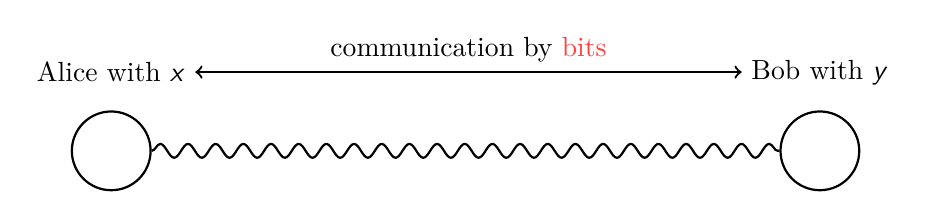
\begin{tikzpicture}[state/.style={circle,draw,thick,minimum size=1cm}]
\node at (0,0) (A) {Alice with $x$};
\node at (9,0) (B) {Bob with $y$};
\node at (0,-1)[state] (A1) {};
\node at (9,-1)[state] (B1) {};
\draw[thick,decorate,decoration=snake] (A1) -- (B1);
\draw[thick,<->] (A) -- node[anchor=south, midway]{communication by \emm{bits}} (B);
\end{tikzpicture}
%\includegraphics[width=30pt]{Alice_in_Wonderland.png}

\vspace{2em}
\begin{center}
Communication complexity of $f$

$=$
the smallest number of transmitted bits for evaluating $f(x,y)$.
\end{center}
\end{frame}
\fi

\begin{frame}{PR box gives a winning probability 1\\{\normalsize [van Dam 2013 {\small (arXiv 2005) (PhD. thesis 1999)} \numc{168}]}}
If the CHSH probability is 1, a winning probability of \emm{any XOR game} is \emm{1} !

\vspace{1em}
Any boolean function can be represented by a $\mathbb{F}_2$-polynomial.
\begin{equation*}
%f(x,y) = \bigoplus_i A_i(x) \wedge B_i(y).
f(x,y) = \bigoplus_z \mathbb{I}\{x = z\} \wedge f(z, y).
\end{equation*}

%\vspace{1em}
%$\mathsf{IP}_n\colon \{0,1\}^n\times\{0,1\}^n\to \{0,1\},\, (x,y) \mapsto \bigoplus_i x_i \wedge y_i$.

%\vspace{1em}
%Since there are measurements satisfying
Recall Alice and Bob have nonlocal boxes with
\begin{equation*}
\Pr(a \oplus b = x\wedge y) = 1
\end{equation*}
for any $(x,y)\in\{0,1\}^2$,
%
\begin{align*}
%\bigoplus_i A_i(x) \wedge B_i(y)
\bigoplus_z \mathbb{I}\{x = z\} \wedge f(z, y)
&= \bigoplus_z (a_z \oplus b_z)\\
&= \left(\bigoplus_z a_z\right) \oplus \left(\bigoplus_z b_z\right).
\end{align*}
\end{frame}

\begin{frame}{Bias}
For a probability $p\in[1/2,1]$, $\delta:=2p-1\in[0,1]$ is called a \emm{bias}.
In other word,
\begin{equation*}
p = \frac{1+\delta}2.
\end{equation*}
%$\delta$ is called a bias.
Let $\emm{\delta}$ be a bias of the CHSH probability $p_\mathsf{CHSH}$.
\begin{itemize}
\item $p_\mathsf{CHSH}=3/4 \iff \delta = 1/2$.
\item $p_\mathsf{CHSH}=(2+\sqrt{2})/4 \iff \delta = 1/\sqrt{2}$.
\item $p_\mathsf{CHSH}=1 \iff \delta = 1$.
\end{itemize}

\vspace{1em}
\begin{itemize}
\item If $X$ is $\pm1$ random variable, the bias (for a prob. of 1) is $\emm{\mathbb{E}[X]} = \frac{1+\delta}2 - \frac{1-\delta}2=\delta$.
\item If $X$ and $Y$ are independent 0-1 random variables with bias (for a prob. of 0) $\delta_X$ and $\delta_Y$, respectively,
the bias of $X\oplus Y$ is $\emm{\delta_X\delta_Y}$.
\end{itemize}


%\begin{itemize}
%\item $f$ is used for a boolean function $\{0,1\}^n\times\{0,1\}^n\to\{0,1\}$.
%\item $g$ is used for a boolean function $\{0,1\}^n\to\{0,1\}$. $g^\oplus$ corresponds to $f$.
%\end{itemize}

\end{frame}

\begin{frame}{Constant winning probability\\{\small [Brassard, Buhrman, Linden, M\'ethot, Tapp, Unger 2006 \numc{250}]}}
%$P_\mathsf{CHSH}>\frac{3+\sqrt{6}}6\approx 0.908$ $\Longrightarrow$ \emm{Trivial} communication complexity on \emm{probabilistic} framework
$p_\mathsf{CHSH}>\frac{3+\sqrt{6}}6\approx 0.908 \iff \delta > \sqrt{\frac23}$

 $\Longrightarrow$ A winning probability of any XOR game is \emm{constant ($> \frac12$)}.




\vspace{1em}
By using shared random bits $r\in\{0,1\}^n$ and Bob's private random bit $r'\in\{0,1\}$,
\begin{align*}
a &= f(x, r)\\
b &= \begin{cases}
0,& \text{if } y = r\\
r',& \text{otherwise.}
\end{cases}
\end{align*}

$a\oplus b = f(x,y)$ with probability
\begin{equation*}
\frac1{2^n} + \left(1-\frac1{2^n}\right)\frac12
=\frac{1+2^{-n}}{2}.
\end{equation*}


%\begin{itemize}
%\item $\mathsf{CHSH}=4$: Trivial communication complexity.
%\item $\mathsf{CHSH}>2+\frac{2}{3}\sqrt{6}\approx 3.633$: Trivial communication complexity on \emm{probabilistic} framework (von Neumann's fault-tolerant computation by $\mathsf{Maj}_3$)
%[Brassard, Buhrman, Linden, M\'ethot, Tapp, and Unger 2006 \numc{227}].
%\end{itemize}
\end{frame}

\begin{frame}{Bias amplification by $\mathsf{Maj}_3$}
\vspace{-.5em}
\begin{align*}
\mathsf{Maj}_3(z_1,z_2,z_3) &= \frac12\left(z_1+z_2+z_3-z_1z_2z_3\right)\\
\mathbb{E}\left[\mathsf{Maj}_3(z_1,z_2,z_3)\right] &= \frac32\epsilon -\frac12\epsilon^3
\end{align*}
\begin{center}
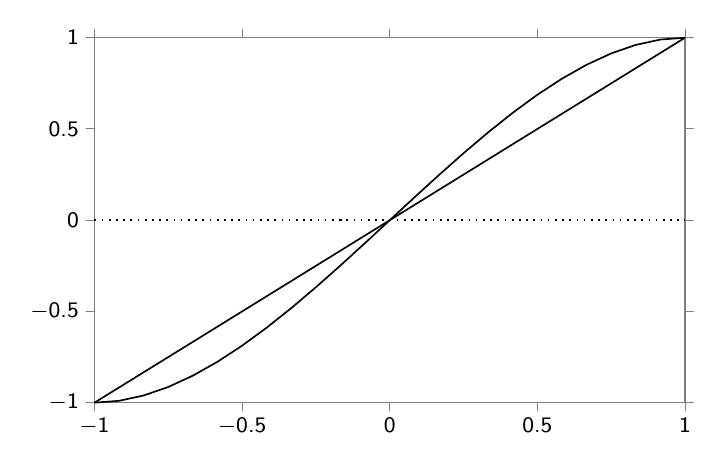
\begin{tikzpicture}[scale=1.5]
\datavisualization[scientific axes, x axis={ticks={few}}, visualize as line/.list={zero,x,maj},
zero={style={dotted}}]
data[set=zero, format=function]{
var x : interval[-1:1];
func y = 0;
}
data[set=x, format=function]{
var x : interval[-1:1];
func y = \value x;
}
data[set=maj, format=function]{
var x : interval[-1:1];
func y = 0.5 * (3 * \value x - \value x * \value x * \value x);
};
\end{tikzpicture}
\end{center}
\end{frame}

\begin{frame}{Bias amplification by noisy $\mathsf{Maj}_3$\newline\normalsize[von~Neumann 1956 \numc{2588}]}
\vspace{-1.5em}
\begin{align*}
\mathsf{Maj}_3(z_1,z_2,z_3) &= \frac12\left(z_1+z_2+z_3-z_1z_2z_3\right)\\
\mathbb{E}\left[\emm{y}\mathsf{Maj}_3(z_1,z_2,z_3)\right] &= \emm{\rho}\left(\frac32\epsilon -\frac12\epsilon^3\right)
\end{align*}
\begin{center}
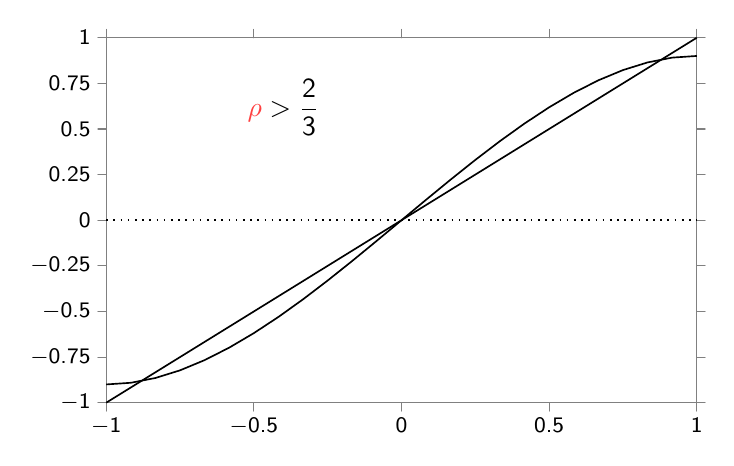
\begin{tikzpicture}[scale=1.5]
\datavisualization[scientific axes, x axis={ticks={few}}, visualize as line/.list={zero,x,maj},
zero={style={dotted}}]
data[set=zero, format=function]{
var x : interval[-1:1];
func y = 0;
}
data[set=x, format=function]{
var x : interval[-1:1];
func y = \value x;
}
data[set=maj, format=function]{
var x : interval[-1:1];
func y = 0.9* 0.5 * (3 * \value x - \value x * \value x * \value x);
}
info {
\draw node at (1.5,2.5)  {$\displaystyle\emm{\rho}>\frac23$};
};
\end{tikzpicture}
\end{center}
\end{frame}

\begin{frame}{Probability of succeeding of computation of $\mathsf{Maj}_3$}
\vspace{-1.0em}
\begin{equation*}
\mathsf{Maj}_3(z_1,z_2,z_3) = z_1z_2 \oplus z_2z_3\oplus z_3z_1
\end{equation*}
\small
\begin{align*}
&\mathsf{Maj}_3(a_1\oplus b_1, a_2\oplus b_2, a_3\oplus b_3)\\
&= (a_1\oplus b_1)(a_2\oplus b_2) \oplus (a_2\oplus b_2)(a_3\oplus b_3) \oplus (a_3\oplus b_3)(a_1\oplus b_1)\\
&=
\emm{(a_1\oplus a_2)(b_2\oplus b_3)} \oplus \emm{(a_2\oplus a_3)(b_1\oplus b_2)}\\
&\qquad \oplus a_1a_2 \oplus a_2a_3 \oplus a_3 a_1\\
&\qquad \oplus b_1b_2 \oplus b_2b_3 \oplus b_3 b_1\\
&=
(\emm{\alpha_0 \oplus \beta_0 \oplus e_0}) \oplus (\emm{\alpha_1\oplus \beta_1 \oplus e_1})\\
&\qquad \oplus a_1a_2 \oplus a_2a_3 \oplus a_3 a_1\\
&\qquad \oplus b_1b_2 \oplus b_2b_3 \oplus b_3 b_1\\
&=\left(\alpha_0 \oplus \alpha_1
\oplus a_1a_2 \oplus a_2a_3 \oplus a_3 a_1\right)
\oplus \left(\beta_0 \oplus \beta_1
\oplus b_1b_2 \oplus b_2b_3 \oplus b_3 b_1\right)
\oplus \emm{e_0 \oplus e_1}.
\end{align*}
\begin{equation*}
%p^2 + (1-p)^2 > \frac{5}{6} \iff p> \frac{3+\sqrt{6}}6\approx 0.908.
\delta^2 > \frac23 \iff \delta > \sqrt{\frac23}\iff p> \frac{1+\sqrt{\frac23}}2=\frac{3+\sqrt{6}}6\approx 0.908.
\end{equation*}
\end{frame}


\section{Generalization of Brassard et al's protocol}



\if0
%\begin{frame}{Summary of this work~~[Mori arXiv:1604.05663, PRA]}
\begin{frame}{Summary of our work\newline\normalsize[Mori Phys.~Rev.~A 94, 052130, 2016]}
First, we
\begin{itemize}
\setlength{\itemsep}{1.5em}
\item show that the best \emm{non-adaptive PR-correct} protocol corresponds to a $\mathbb{F}_2$-polynomial representation.
\item show a particular adaptive protocol better than any non-adaptive PR-correct protocol inspired by the paper on \emm{information causality} {\small [Paw\l owki, Paterek, Kaszlikowski, Scarani, Winter, Zukowki 2009 \numc{324}]}.
\end{itemize}

\vspace{1em}
We then show
\begin{itemize}
\item On the basis of Brassard et al.'s idea, we \emm{cannot improve the threshold}, i.e., the 3-input majority is the optimal function for the bias amplification.
\end{itemize}
\end{frame}
\fi

\begin{frame}{Generalization of Brassard et al's protocol}
\begin{itemize}
\setlength{\itemsep}{3.0em}
\item Why $\mathsf{Maj}_3$ ?
\item Replace $\mathsf{Maj}_3$ with arbitrary boolean function.
\item Two important parameters: 
\begin{itemize}
\item $2$: Number of nonlocal boxes for the computation.
\item $2/3$: Threshold for the bias amplification.
\end{itemize}
\item We showed that the $\mathsf{Maj}_3$ is \emm{the unique optimal function} in a simple generalization~[Mori, Phys.~Rev.~A 94, 052130, 2016].
\end{itemize}
\end{frame}

\begin{frame}{Information causality}
{\small [Paw\l owki, Paterek, Kaszlikowski, Scarani, Winter, Zukowki 2009 \numc{375}]}
Information causality: 
\begin{center}
\bfseries
If Alice communicates $\mathbf{m}$ bits to Bob,
the total information obtainable by Bob cannot be greater than $\mathbf{m}$.
\end{center}

\vspace{2em}
Alice has $2^n$ bits. Bob wants to know one of Alice's $2^n$ bits.
Alice doesn't know which bit Bob wants to know.

\vspace{1em}
IC says that Alice has to send $2^n$ bits.

\vspace{2em}
\centering
Above the quantum limit $0.854$, Alice only has to send $1.99^n$ bits.
\end{frame}

\begin{frame}{Address function}
\small
\begin{align*}
\mathsf{Addr}_n(x_0,\dotsc,x_{2^n-1},y_1,\dotsc,y_n) := x_y
\end{align*}
where $y:= \sum_{i=1}^n y_i 2^{i-1}$.
\begin{theorem}[{\scriptsize [Paw\l owski, Paterek, Kaszlikowki, Scarani, Winter, Zukowski 2009 \numc{375}]}]
There is an adaptive protocol of the XOR game for the address function with bias \emm{$\delta^n$}.
\end{theorem}
\begin{block}{Proof}
Induction.

For $n=1$, from
\begin{equation*}
\mathsf{Addr}_1(x_0,x_1,y_1) = x_0 \oplus y_1 (x_0\oplus x_1)
\end{equation*}
there is a non-adaptive protocol with bias $\delta$.
\end{block}
\end{frame}

\begin{frame}{Address function}
\begin{proof}[Proof (Cont'd)]
\begin{equation*}
\mathsf{Addr}_n(x_0,\dotsc,x_{2^n-1},y_1,\dotsc,y_n) =
\mathsf{Addr}_1(z_0,z_1,y_n)
\end{equation*}
where
\begin{align*}
z_0 &:= \mathsf{Addr}_{n-1}(x_0,\dotsc,x_{2^{n-1}-1},y_1,\dotsc,y_{n-1})\\
z_1 &:= \mathsf{Addr}_{n-1}(x_{2^{n-1}},\dotsc,x_{2^{n}-1},y_1,\dotsc,y_{n-1}).
\end{align*}
\begin{align*}
&\mathsf{Addr}_1(z_0,z_1,y_n) =
\mathsf{Addr}_1(a_0\oplus b_0\oplus e_0,a_1\oplus b_1\oplus e_1,y_n)\\
&=\mathsf{Addr}_1(a_0,a_1,y_n) \oplus b_{y_n} \oplus e_{y_n}\\
&=a'\oplus b'\oplus e'
 \oplus b_{y_n} \oplus e_{y_n}\\
&=a' \oplus (b'\oplus b_{y_n}) \oplus (e' \oplus e_{y_n}).
\end{align*}
This protocol has bias \emm{$\delta^n$}.
\end{proof}
\end{frame}

\begin{frame}{Repetition}
The 1 bit communication has error probability $\epsilon:= \frac{1-\delta^n}2$.\\
The $m$ bits communication has error probability
$\le \left(2\sqrt{\epsilon(1-\epsilon)}\right)^m$.

\vspace{1.5em}
From
\begin{equation*}
\left(2\sqrt{\epsilon(1-\epsilon)}\right)^m
=(1-\delta^{2n})^{\frac{m}2}
\end{equation*}
error probability goes to zero if
\begin{equation*}
m \gg \emm{\delta}^{\emm{-2}n}.
\end{equation*}
If $\delta>1/\sqrt{2}$, then $\emm{\delta^{-2}}<2$.

\vspace{1em}
\begin{center}
If CHSH probability is greater than the quantum limit,

\vspace{.5em}
\bfseries
$\mathbf{1.99^n}$ bits communication allows Bob to select arbitrary one bit from Alice's $\mathbf{2^n}$ bits.
\end{center}
\end{frame}


\end{document}
